Previous chapters addressed the problem of robotic motion planning and control by leveraging techniques from control theory and optimal control. In particular, these techniques were used to generate open and closed-loop control laws to accomplish specific tasks such as trajectory generation, trajectory tracking, and stabilization or regulation about a particular robot state. One common component among all of these algorithms was the use of a model of the robot's kinematics or dynamics, which mathematically defines how the robot transitions from state to state based on control inputs.

In this chapter yet another set of algorithms for motion planning/trajectory generation is discussed\cite{LaValle2006}. These algorithms are particularly well suited for higher-level motion planning tasks, such as motion planning in environments with obstacles. This is accomplished by focusing on formulating the motion planning problem for a robot with respect to the robot's \textit{configuration space} rather than the \textit{state space} that was used in previous chapters. While the robot's configuration is derivable from its state (and still characterizes all of the robot's degrees of freedom), the definition of the configuration space can be useful because it can be tailored to collision avoidance tasks\footnote{In some cases the choice of configuration and state may end up being the same.}.
Historically speaking, these approaches were developed alongside many of the techniques from previous chapters, and are still being researched today.

\notessection{Search-Based Motion Planning}
Recall the general definition of the motion planning problem:
\begin{definition}[Motion planning problem]
Compute a sequence of actions to go from an initial condition to a terminal condition while respecting constraints and possibly optimizing a cost function.
\end{definition}
Previous chapters approached this problem by formulating mathematical optimization problems that minimized a cost function subject to constraints on the motion (i.e. from dynamics/kinematics, control limits, or conditions on the robot's state), or leveraged differential flatness properties of the model. In these approaches, the robot's trajectory was parameterized by its state $\x$ and the corresponding control inputs $\bu$ which satisfied a set of differential equations
\begin{equation*}
    \dot{\x} = f(\x, \bu).
\end{equation*}

In this chapter, the motion planning problem will instead be addressed with respect to a \textit{configuration space} ($C$-space).
The configuration $\q$ of a robot is derivable from the full dynamics state $\x$ and captures all of the degrees of freedom of the robot (i.e. all rigid body transformations). In some cases the state and configuration of the robot may be the same, but in other cases the definition of the configuration can be tailored to simplify the motion planning problem. One important example of this is for \textit{geometric path planning}, where paths in the configuration space can be planned without considering the robot kinematic/dynamics model.

\begin{example}[Motivating Example] \label{ex:mot}
\theoremstyle{definition}
Consider the L-shaped robot from Figure \ref{fig:2dworkspace} that lives in a 2D world with obstacles, and is trying to get from one point to another. Additionally, suppose this robot has a state $\x = [x,y,\theta,\dot{x}, \dot{y}, \dot{\theta}]^\top $, and consider a configuration space defined by $\q = [x,y,\theta]^\top $ which fully captures the robot's degrees of freedom. Since the motion planning problem in this case involves obstacle avoidance, it might be easier to just plan a sequence of configurations $\q$ that are collision free (as is shown in the right-side graphic of Figure \ref{fig:2dworkspace}).

In this case, the use of the configuration space has simplified the motion planning problem by abstracting away the consideration of the robot's dynamics. Once the geometric path has been defined in configuration space, other techniques (such as those discussed in previous chapters) could be used to perform lower-level control functions for path tracking.
\begin{figure*}[ht] 
    \centering 
    \includegraphics[width=0.85\linewidth]{tex/figs/ch05_figs/2d_ws_obstacles.png}
    \caption{Motivating example: motion planning in a 2D workspace with obstacles.}
    \label{fig:2dworkspace} 
\end{figure*}

Additionally, it is important to note that the $C$-space is a subset of $\R^3$, and in particular the $C$-space is $\R^2 \times \mathcal{S}^1$. This subspace is special because it includes the \textit{manifold} $\mathcal{S}^1$, which characterizes the fact that the rotational degree of freedom $\theta$ satisfies $\theta = \theta \pm 2\pi k$ for all $k = 1,2,\dots$. This distinction is important to make because it endows the planner with the ability to move from one angle to another in two different ways (i.e. the robot can turn left or turn right). For example, suppose the robot in Figure \ref{fig:2dworkspace} has a current heading of $\theta_0$ and wants move to have a heading $\theta_g$ subject to the constraint of avoiding a $\C$-space obstacle (see Figure \ref{fig:rotational-dof-fig}). If the equivalence between the angles 0 and $2\pi$ is not established in the definition of the configuration space, the robot would not be able to traverse a collision-free path to the desired heading in the configuration space (see red trajectory). Instead, since the configuration space is defined with respect to $\Space^1$, the robot is able to achieve the desired heading (see green trajectory).

\begin{figure}[h]
\begin{center}
\includegraphics[width=0.9\textwidth]{tex/figs/ch05_figs/S1_obstacle.png}
\caption{Example trajectory planning where the description of the configuration space using the manifold $\Space^1$ is crucial to path planning. In particular, rotating clockwise leads to collision but rotating counter-clockwise is a feasible path.}
\label{fig:rotational-dof-fig}
\end{center}
\end{figure}

\end{example}

In this chapter two types of motion planning algorithms that plan in the configuration space will be discussed. The first class consists of \textit{grid-based methods}, and the second class consists of methods referred to as \textit{combinatorial planners}.


\subsection{Grid-based Motion Planners}
Suppose the robot's configuration $\q$ is a $d$ dimensional vector, then the $C$-space is a subset of $\R^d$. Critically, this is a continuous space and therefore there are an infinite number of potential configurations the robot could be in. To simplify this problem, grid-based motion planners use a grid to discretize the $C$-space into a finite number of allowable configurations. For example, in a simple $C$-space in two dimensions the grid might look like that shown in Figure \ref{fig:grid}.
\begin{figure}[ht] 
    \centering 
    \includegraphics[width=0.65\linewidth]{tex/figs/ch05_figs/2d_ws_grid.png}
    \caption{Discretizing the configuration space using a grid.}
    \label{fig:grid} 
\end{figure} 
In grid-based planners, undesirable configurations are simply represented by identifying some cells of the grid to be forbidden (e.g. for obstacle avoidance). The dynamics/kinematics of the robot are also abstracted away and it is assumed that the robot has the ability to move freely between adjacent cells (configurations).
After this discretization, the resulting motion planning problem is sometimes referred to as a \textit{discrete planning} problem because only a finite number of options are available at each step, and only a finite number of configurations are possible. The planning problem then reduces to finding a way to traverse through the cells from the initial configuration to a desired final configuration.

Mathematically, problems of this type are commonly expressed using discrete \textit{graphs}. A graph $G = (V,E)$, is simply defined by a set of vertices $V$ and a set of edges $E$. In the context of grid-based motion planners, each vertex $v \in V$ represents a \textit{free} cell of the grid, and each edge $(v,u) \in E$ corresponds to a connection between adjacent cells. With the graph representation, the planning problem is to find a way to traverse through the graph to reach the desired vertex. Algorithms for solving such problems are referred to as \textit{graph search methods}.

The advantages of such approaches are that they are simple and easy to use, and for some problems can be very fast. The disadvantages are primarily the result of the discretization procedure. In some cases, if the resolution of the grid is not fine enough the search algorithm may not always be able to find a solution. Additionally, for a fixed resolution the size of the graph grows exponentially with respect to the dimension of the configuration space. Therefore this approach is generally limited to simple robots with a low-dimensional configuration space.

\subsubsection{Label Correcting Algorithms}
Since the graph is defined by a \textit{finite} number of vertices (also referred to as \textit{nodes}) and edges, it should be theoretically possible to solve a graph search problem in finite time. However in order to achieve this in practice, several simple ``accounting'' tricks need to be used to keep track of how the search has progressed and to avoid redundant exploration. Additionally, it is desirable to find a ``best'' path, and so a mechanism for keeping track of the current best path is required during the search.

A general set of algorithms known as \textit{label correcting algorithms} employ such accounting techniques to guarantee good performance. In these algorithms, the notion of a ``best'' path is logged in terms of a cost-of-arrival.
\begin{definition}[Cost-of-Arrival]
The cost-of-arrival associated with a vertex $q$ with respect to a starting vertex $q_I$ is the cost associated with taking the best known route from $q_I$ to $q$ along edges of the graph, and is denoted $C(q)$. 
\end{definition}
Additionally, in a slight abuse of notation the cost from traversing an edge from vertex $q$ to vertex $q'$ is denoted as $C(q,q')$. To keep track of what nodes have already been visited and which still need further exploration, label correcting algorithms define a set of \textit{frontier vertices} (sometimes also referred to as \textit{alive}). This allows guarantees to be made that the search algorithm will avoid redundant exploration, and will terminate in finite time. It also guarantees that if a path from the initial vertex $q_I$ to the goal vertex $q_G$ exists, that it will be found.

In general, label correcting algorithms take the following steps to find the best path from an initial vertex $q_I$ to a desired vertex $q_G$\footnote{In terms of robot motion planning this would be a search over paths through the discretized configuration space. Therefore the vertices of the graph are referred to as $q$ to better connect this abstraction with their physical interpretation being a particular robot configuration $\q$.}:

\begin{enumerate}
    \item Initialize the set of frontier vertices as $Q = \{q_I\}$ and set $C(q_I) = 0$. Initialize the cost-of-arrival of all other vertices $q'$ as $C(q') = \infty$.
    \item Remove a vertex from $Q$ and explore each of its connected vertices $q'$. For each $q'$, determine the candidate cost-of-arrival $\tilde{C}(q')$ associated with moving from $q$ to $q'$ as $\tilde{C}(q') = C(q) + C(q,q')$. If the candidate cost-of-arrival $\tilde{C}(q')$ is lower than the current cost-of-arrival $C(q')$ AND is lower than the current cost-of-arrival $C(q_G)$, then set $C(q') = \tilde{C}(q')$, define $q$ as the parent of $q'$, and add $q'$ to the set $Q$ if $q'$ is not $q_G$.
    \item Repeat step 2 until the set of frontier vertices $Q$ is empty. 
\end{enumerate}

The bulk of the work is done is Step 2. In particular, for the selected $q$ from $Q$, these algorithms search its connected neighbors $q'$ to see if moving from $q$ to $q'$ will lead to a lower overall cost than previously found paths to $q'$. This is why the algorithms are called ``label correcting'', since they ``correct'' the cost-of-arrival as better paths are found throughout the search process. Eventually, once the best path from $q_I$ to $q$ is found, $q$ will never again be added to the set $Q$ and therefore the algorithm is guaranteed to eventually terminate.

\begin{theorem}[Label Correcting Algorithms]
If a feasible path exists from $q_I$ to $q_G$, then the label correcting algorithm will terminate in finite time with
$C(q_G)$ equal to the optimal cost of traversal, $C^*(q_G)$.
\end{theorem}

The primary way in which label correcting algorithms differ from each other is in how they select the next vertex $q$ from the set of frontier nodes $Q$. In fact, the set $Q$ is often referred to as a \textit{priority queue} since the algorithm might assign priority values to the order in which vertices are selected. Different approaches for prioritizing include \textit{depth-first search}, \textit{breadth-first search}, and \textit{best-first search}.

\paragraph{Depth-First Search}
Depth-first search in a directed graph expands each node up to the deepest level of the graph, until a chosen node has no more successors. Another way to think about this in terms of the set $Q$ is ``last in/first out'', where whenever a new vertex $q$ is selected from $Q$ it chooses those vertices that were most recently added.

\begin{marginfigure}
\begin{center}
\includegraphics[width=0.95\textwidth]{tex/figs/ch05_figs/depth_first.PNG}
\caption{Depth-First Search}
\end{center}
\end{marginfigure}

\paragraph{Breadth-First Search}
Breadth-first search begins with the start node and explores all of its neighboring nodes. Then for each of these nodes, it explores all their unexplored neighbors and so on. In terms of $Q$, this is like storing the frontier nodes as a queue with the first node added is the first node selected.

\begin{marginfigure}
\begin{center}
\includegraphics[width=0.95\textwidth]{tex/figs/ch05_figs/breadth_first.PNG}
\caption{Breadth First Search}
\end{center}
\end{marginfigure}

\paragraph{Best-First Search}
Also commonly known as \textit{Dijkstra’s algorithm}, this approach greedily selects vertices $q$ from $Q$ by looking at the current best cost-of-arrivals. Mathematically,
\begin{equation*}
   q = \textrm{arg} \min_{q \in Q} C(q).
\end{equation*}
This approach is sometimes considered an ``optimistic'' approach since it is essentially making the assumption that the best current action will always correspond to the best overall plan.
In practice this approach typically provides a more efficient search procedure relative to depth-first or breadth-first approaches because it can account for the cost of the path, however additional improvements can be made.

\subsubsection{A* Algorithm}
A* is a label correcting algorithm that is a modified version of Dijkstra's algorithm. In Dijkstra's algorithm the goal vertex $q_G$ is not taken into account, potentially leading to wasted effort in cases where the greedy choice makes no progress towards the goal. This is quantified by a quantity called the \textit{cost-to-go}.

\begin{definition}[Cost-to-Go]
The cost-to-go associated with a vertex $q$ with respect to a goal vertex $q_G$ is the cost associated with taking the best known route from $q$ to $q_G$ along edges of the graph.
\end{definition}
In practice, the cost-to-go is not usually known, and therefore \textit{heuristics} are used to provide approximate cost-to-go values $h(q)$. In order for the heuristic to be useful, it must be a positive \textit{underestimate} of the true cost-to-go. An example of a heuristic $h$ is to simply use distance to the goal.

While Djikstra's algorithm only prioritizes a vertex $q$ based on its cost-of-arrival $C(q)$, A* prioritizes based on cost-of-arrival $C(q)$ plus an approximate cost-to-go $h(q)$. This provides a better estimate of the total quality of a path than just using the cost-of-arrival alone. The A* algorithm is defined in Algorithm \ref{alg:astar}.
\begin{algorithm}[ht]\caption{A* Algorithm} \label{alg:astar}
	\KwData{$q_{I}$, $q_{G}$, $G$}
	\KwResult{path}
	$C(q) = \infty, \:\: f(q) = \infty, \:\:  \forall q$ \\
	$C(q_I) = 0$, $f(q_I) = h(q_I)$ \\
	$Q = \{q_I\}$ \\
	\While{$Q$ is not empty}{
	    $q = \argmin_{q' \in Q}f(q')$ \\
	    \If{$q = q_{G}$}{
	        \Return{path}
	    }
	    $Q$.remove($q$)\\
	    \For{$q' \in \{q' \: | \: (q,q') \in E\}$}{
	        $\tilde{C}(q') = C(q) + C(q,q')$ \\
	        \If{$\tilde{C}(q') < C(q')$}{
	        $q'$.parent = $q$\\
	        $C(q') = \tilde{C}(q')$\\
	        $f(q') = C(q') + h(q')$\\
	        \If{$q' \not\in Q$}{
	            $Q$.add($q'$) \\
	        }
	        }
	    }
	}
	\Return{failure}
\end{algorithm}
Note that in the case that the heuristic is chosen to be $h(q) = 0$ for all $q$ then A* is the same as Djikstra's algorithm.


\subsection{Combinatorial Motion Planning} 
Combinatorial approaches to motion planning find paths through the continuous configuration space without resorting to discretizations like in grid-based planners. Recall that in grid-based planners, cells in the discretized configuration space that were undesirable were blocked out and simply not considered in the resulting path search. However, in the case of combinatorial planners the structure of the free portion of the configuration space is considered in a different way.

\begin{figure}[ht]
 \centering
 	\includegraphics[width=.5\textwidth]{tex/figs/ch05_figs/obs_padding.png}
	\caption{Free (white) and forbidden spaces (grey and red) of the configuration space for a simple circular robot in a 2D world. Note that the forbidden space accounts for the physical dimensions of the robot.}
 \label{fig:collision-free-space-fig}
\end{figure}
\begin{figure}[ht]
\begin{center}
\includegraphics[width=0.75\textwidth]{tex/figs/ch05_figs/2d_ws_Cfree.png}
\caption{Once the free (white) and forbidden (grey and red) configurations have been identified, the physical dimensions of the robot can be ignored. This figure shows an example of a path planning problem in $C$-space with obstacles.}
\label{fig:combinatorial-planning}
\end{center}
\end{figure}
First, the subset of the configuration space $C$ that is free (i.e. results in no collisions) is denoted as $C_{free}$ and is called the \textit{free space} (see Figures \ref{fig:collision-free-space-fig} and \ref{fig:combinatorial-planning}).
Combinatorial motion planning approaches operate by computing \textit{roadmaps} through the free space $C_{free}$. A roadmap is a graph $G$ where each vertex represents a point in $C_{free}$ and each edge represents a path through $C_{free}$ that connects a pair of vertices. The set $S$ is then defined for a particular roadmap graph $G$ as the set of all points in $C_{free}$ that are either vertices of $G$ or lie on any edge of $G$.
This graph structure is similar to that used in grid-based planners, with the important distinction that the vertices can potentially be \textit{any} configuration $q \in C_{free}$ while in grid-based planners the vertices are defined ahead of time by discretization. This distinction is very important because the flexibility of choosing the vertices does not result in any loss of information!
Once the roadmap has been defined, a path can be defined by first connecting the initial configuration $q_I$ and goal configuration $q_G$ to the roadmap and then solving a discrete graph search over the roadmap graph $G$.

In general combinatorial planners are \textit{complete} (i.e. the algorithm will either find a solution or will correctly report that no
solution exists), and can even be optimal in some cases. However, often times in practice they are not computationally feasible to implement except in problems with low-dimensional configuration spaces and/or simple geometric representations of the environment. Additionally, it requires that the free space be completely defined in advance, which is not necessarily a realistic requirement.

\subsubsection{Cell Decomposition}
One common approach for deriving the roadmap is to use \textit{cell decomposition} to decompose $C_{free}$.
Cell decomposition refers to the process of partitioning $C_{free}$ into a finite set of regions called cells, which should generally satisfy:
\begin{itemize}
    \item Each cell should be easy to traverse and ideally convex.
    \item Decomposition should be easy to compute.
    \item Adjacencies between cells should be straightforward to determine, in order to build the roadmap.
\end{itemize}

\begin{example}[2D Cell Decomposition] \label{ex:celldecomp}
Consider a two-dimensional configuration space as shown in Figure \ref{fig:cell-decompsition}. This space is decomposed into cells that are either lines or trapezoids by a process called vertical cell decomposition. Once the cells have been defined, the roadmap is generated by placing a vertex in each cell (e.g. at the centroid) as well as a vertex on each shared edge between cells.

If the forbidden space is polygonal, cell decomposition methods work pretty well and each cell can be made to be convex. In general, there exist several approaches for performing cell decomposition. However, cell decomposition in higher dimensions becomes increasingly challenging.

\begin{figure}[ht]
\begin{center}
\includegraphics[width=0.74\textwidth]{tex/figs/ch05_figs/2d_cell_decomp.png}
\caption{Example of 2D Cell Decomposition with $C_{free}$ colored white. A roadmap is defined as the graph $G$ with vertices shown as black dots and edges connecting them. To solve a planning problem with $q_{start}$ and $q_{goal}$ these points are first connected to the roadmap, and then the path is easily defined.}
\label{fig:cell-decompsition}
\end{center}
\end{figure}
\end{example}

\subsubsection{Other Roadmaps}
Other ways to define roadmaps besides using cell decomposition exist. Two possible examples include a maximum clearance or minimum distance approach. Maximum clearance roadmaps simply try to always keep as far from obstacles as possible, for example by following the centerline of corridors. These roadmaps are also sometimes referred to as ``generalized Voronoi diagrams''. Minimum distance roadmaps are generally the exact opposite of maximum clearance roadmaps in that they tend to graze the corners of the forbidden space. In practice this is likely not desirable and therefore these approaches are less commonly used (without modification).

\subsection{Exercises}
\subsubsection{A* Motion Planning}
Complete \textit{Problem 1: A* Motion Planning} located in the online repository:

\vspace{\baselineskip}

\url{https://github.com/PrinciplesofRobotAutonomy/AA274A_HW2},

\vspace{\baselineskip}

where you will implement the A* grid-based motion planning algorithm for some simple 2D environments.
